\begin{frame}
	\frametitle{Introduction}

	\begin{columns}
		\column{0.5\textwidth}
			\begin{center}
				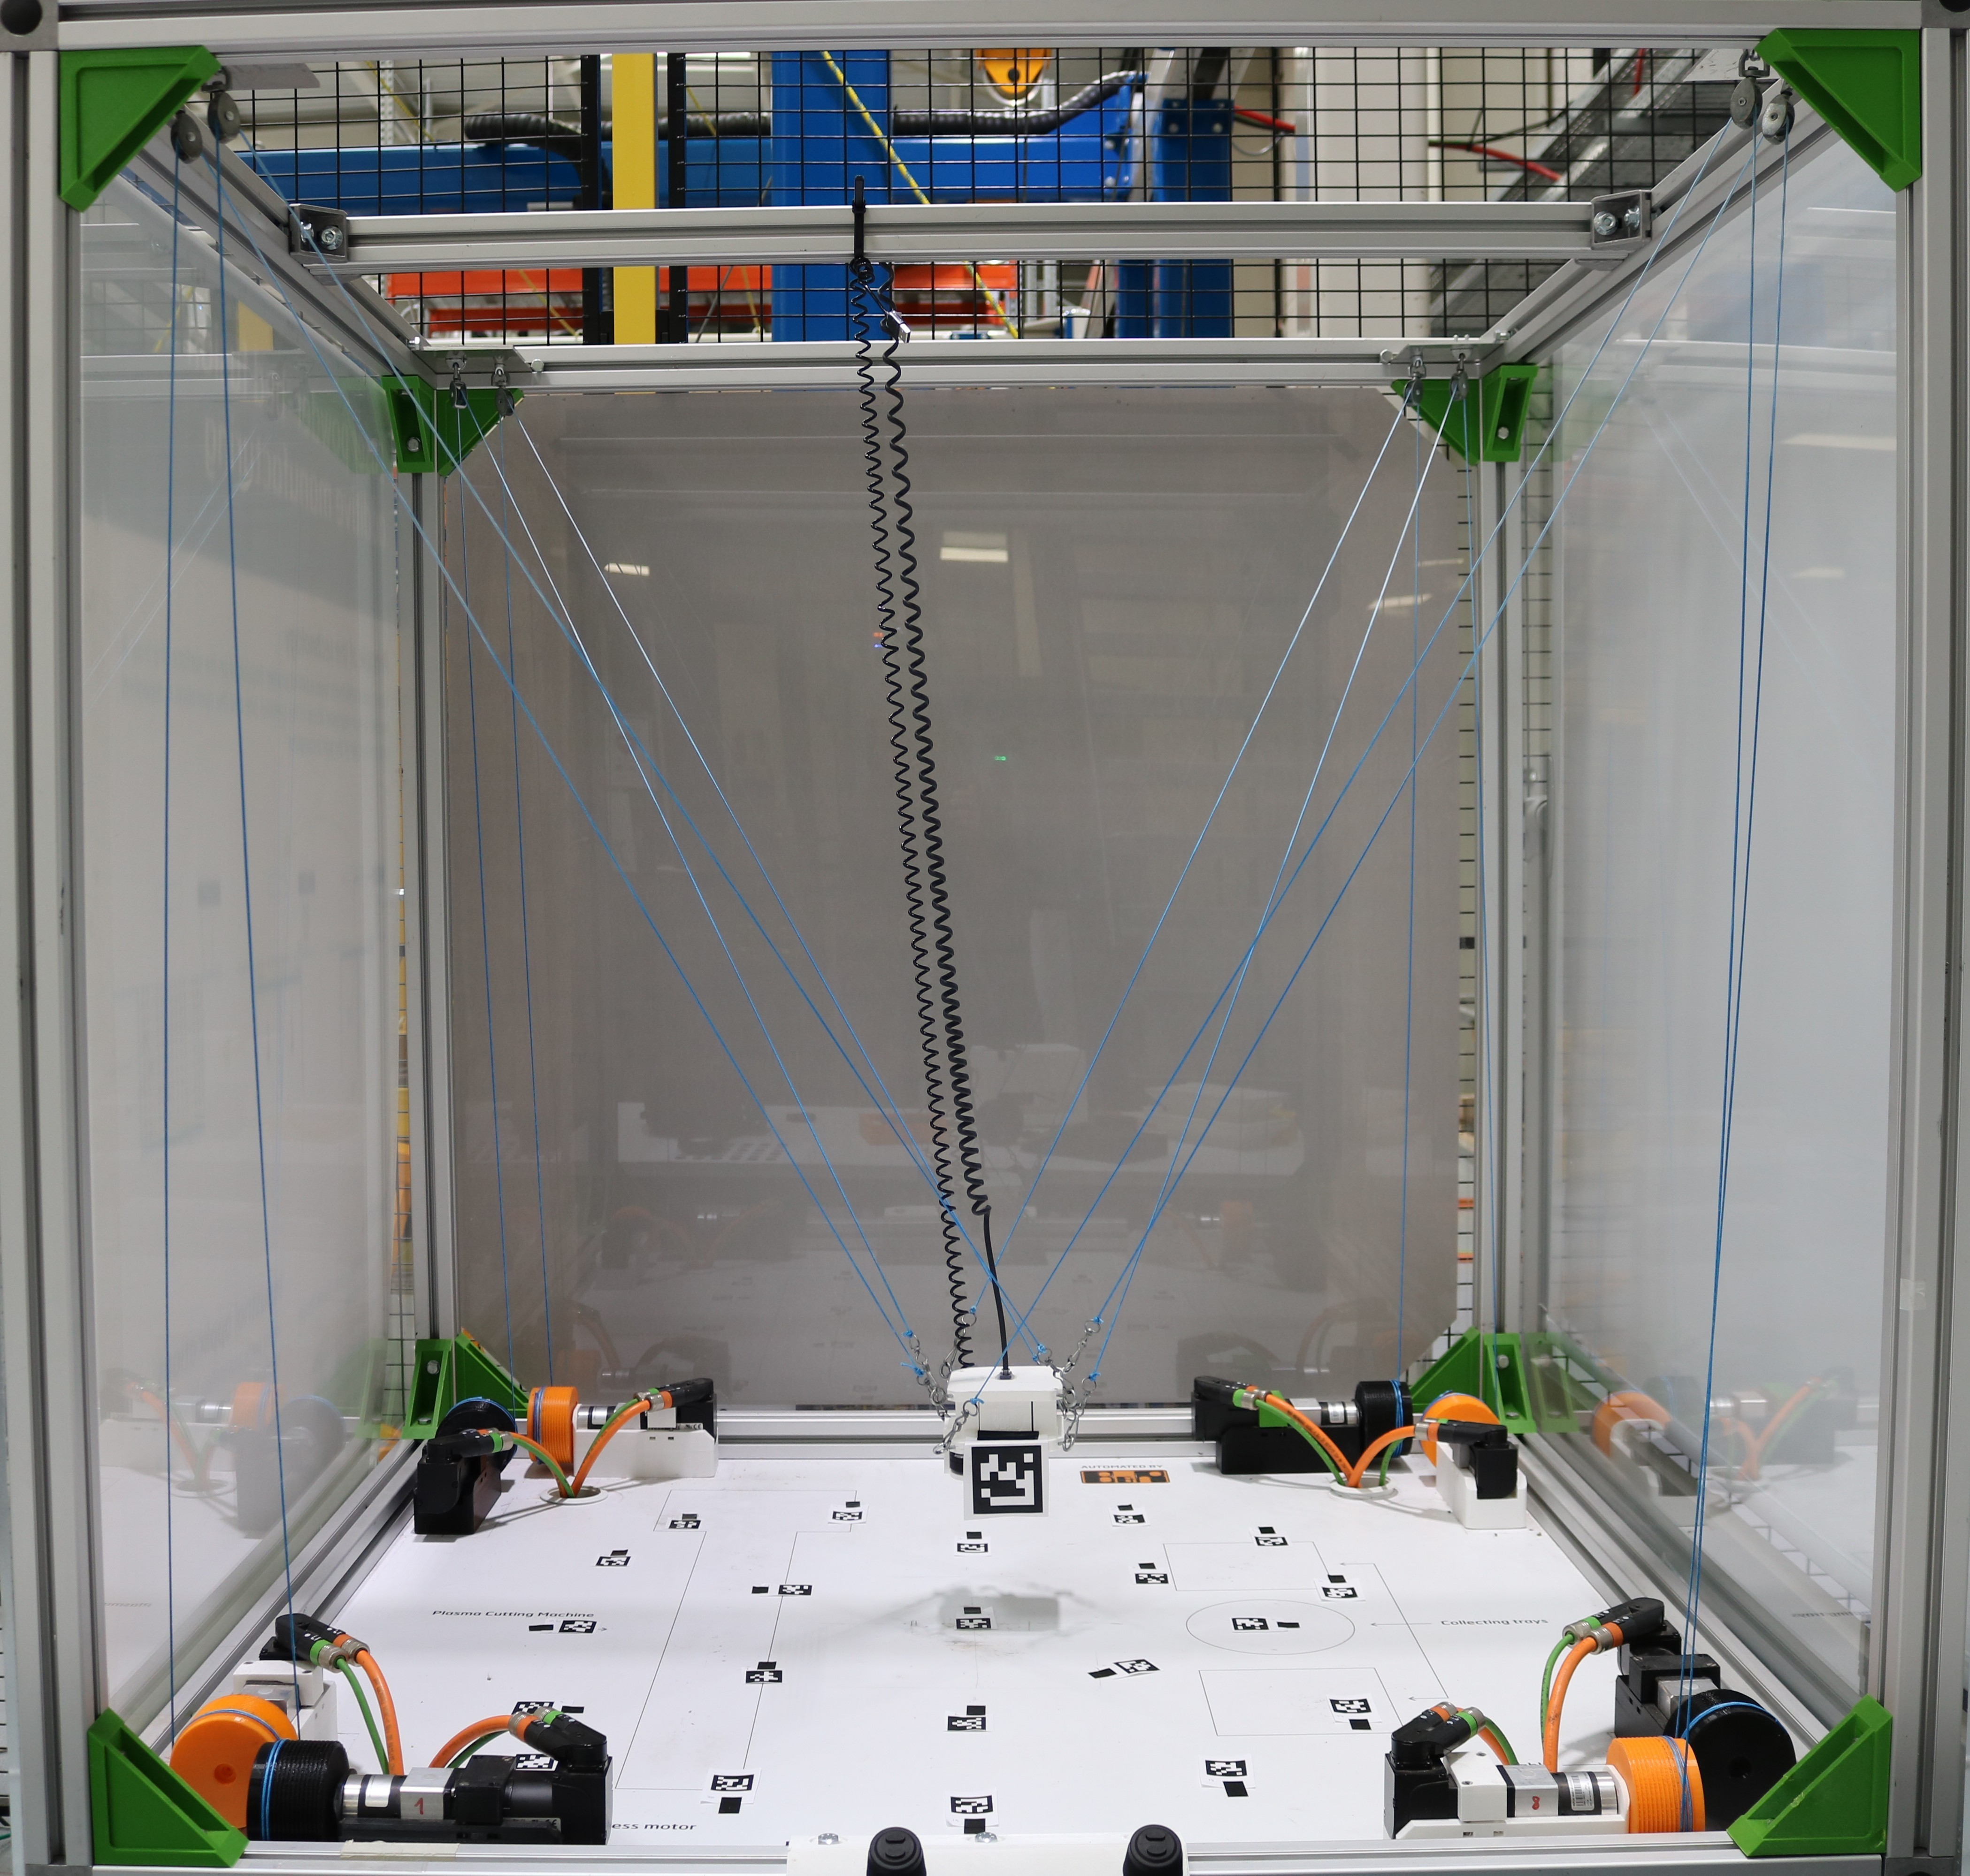
\includegraphics[width=\textwidth]{acrobotHD}
				\captionof{figure}{Acrobot}
			\end{center}

		\column{0.5\textwidth}

			Goals:

			\begin{itemize}

				\item
					Path planning in presence of obstacles

				\item
					Generate smooth trajectories

					\begin{itemize}
						\item High degree of differentiability
						\item High degree of geometric differentiability
					\end{itemize}

				\item
					Adhere to actuator limits

			\end{itemize}
	\end{columns}
\end{frame}

\begin{frame}
	\frametitle{Overview}

	\begin{columns}
		\column{0.75\textwidth}
			\begin{minipage}{\textwidth}
				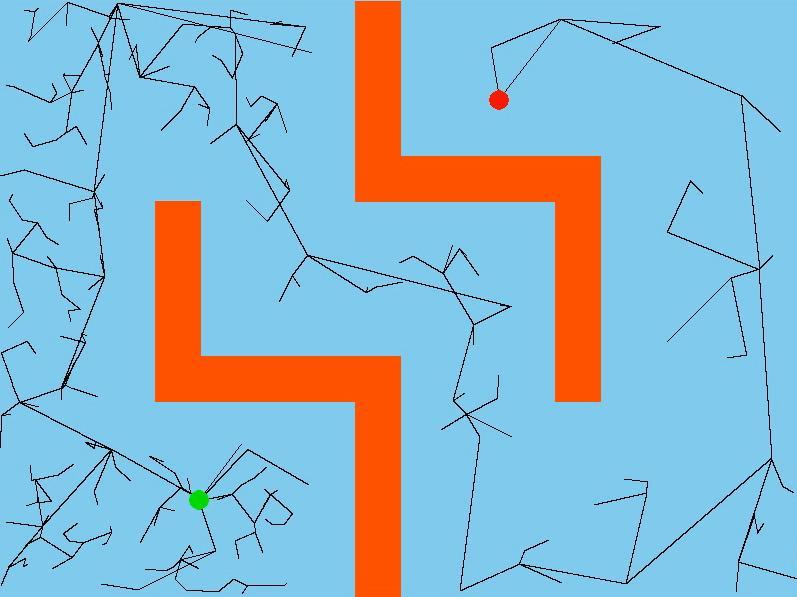
\includegraphics[width=0.5\textwidth]{2d_search_1}%
				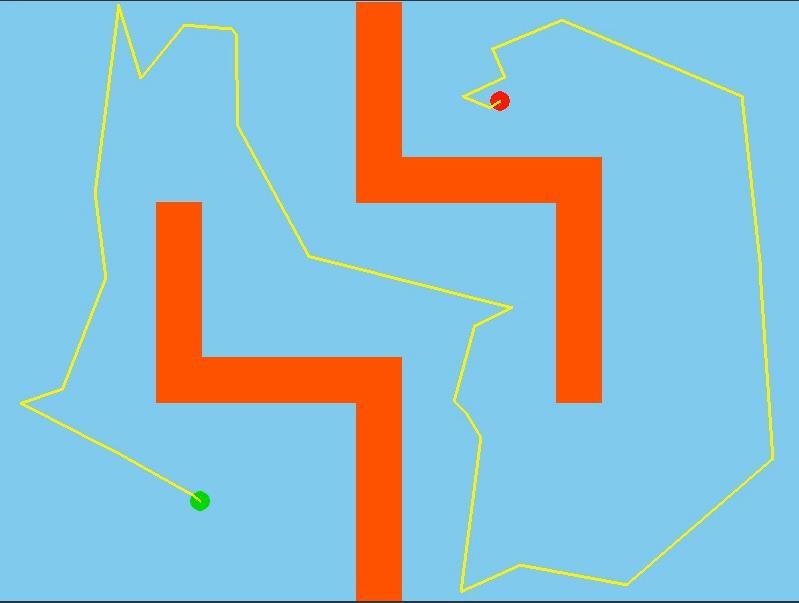
\includegraphics[width=0.5\textwidth]{2d_search_2}
				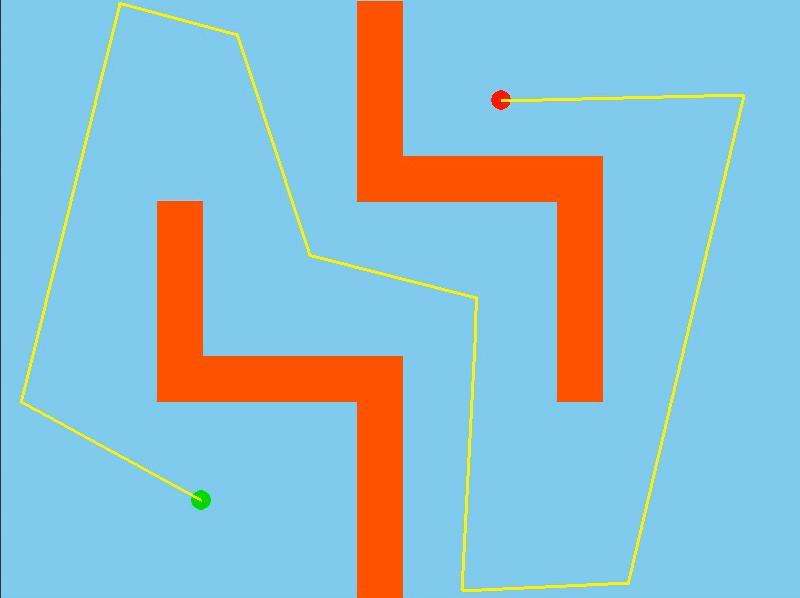
\includegraphics[width=0.5\textwidth]{2d_search_3}%
				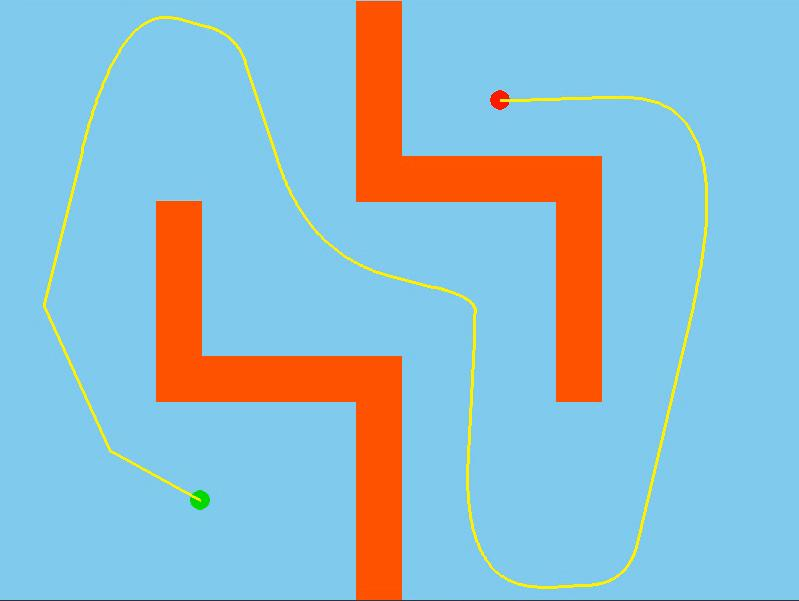
\includegraphics[width=0.5\textwidth]{2d_search_4}
				%\captionof[figure]{Path Planning Overview}
			\end{minipage}

		\column{0.25\textwidth}

			Approach followed:

			\begin{itemize}

				\item

					RRT-based algorithm finds initial path

				\item

					Post-processing steps to simplify and smooth final path

			\end{itemize}

	\end{columns}

\end{frame}

\begin{frame}
	\frametitle{2D Demo}

	\movie[
		height = 5cm,
		width = 5cm,
		externalviewer,
		showcontrols
	]
	{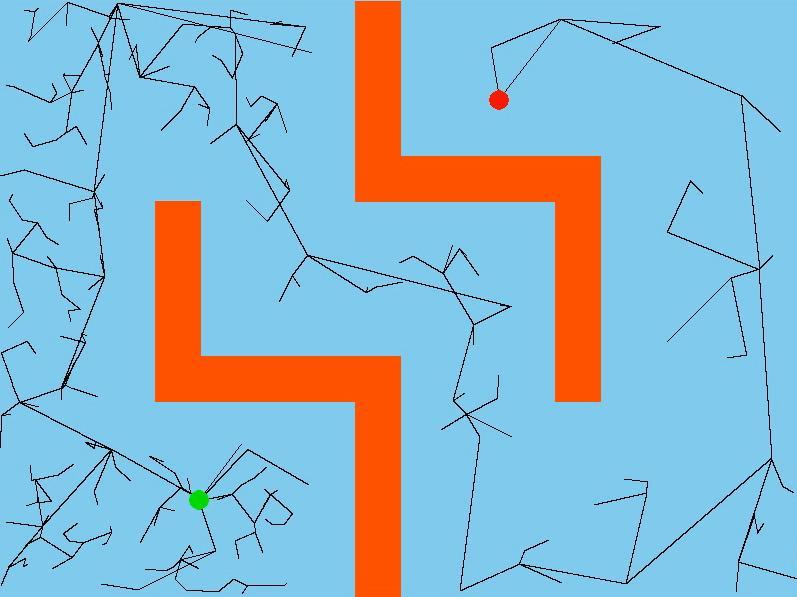
\includegraphics[width=5cm]{2d_search_1}}{./demos/2d_bezier_demo.mp4}
\end{frame}
